\chapter{String Processing}

\section{Regular Expressions}

\subsection{Regular Expressions}

\subsection{Zero-width Lookahead Technique}
\label{sec:lookaroundsplitting}

\begin{figure}
    \centering
    % Wikipedia Public Domain image
    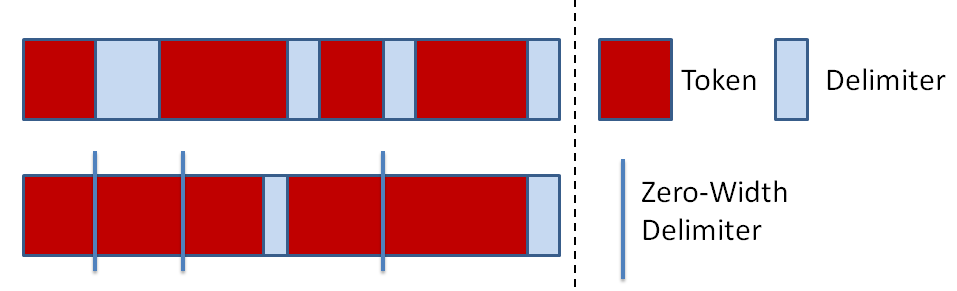
\includegraphics[height=1.5in]{lookaheadsplitting.png}
    \caption{Lookahead Splitting. The top shows a traditional scanner/split which consumes delimiters.
    The bottom shows a scanner using delimiter expressions that may or may not consume characters.}
    \label{fig:lookaheadsplit}
\end{figure}

In some problems (notably, 
      2007/B/Mobile~\ref{sec:2007-b-mobile}, 
      2007/D/Witness~\ref{sec:2007-d-witness}, 
      and 2008/G/Stems~\ref{sec:2008-g-stems}),
the string and/or input handling of these problems can greatly 
benefit from using zero-width positive lookahead/lookbehind regular expressions.

To understand how they work, consider how java.util.Scanner works. By
default, a Scanner splits the input stream into tokens using a delimiter
pattern. The default delimiter pattern is one or more whitespaces
(written as \verb!\p{javaWhitespace}! or, when embedded in Java code, as
\verb!"\\p{javaWhitespace}+"!). The input characters that are matched by the
delimiter itself are consumed by the Scanner – there is no way to
retrieve them.

In some cases, whitespace is not a suitable delimiter. Suppose
you're asked to parse an arithmetic expression that uses +, -, *,
and /. Whitespaces are optional, so both \verb!1+1! and \verb!1 + 1! as well as 
\verb!1 +1! are valid expressions. If you made the operators '+', '-'
etc. delimiters (perhaps in addition to whitespace), a Scanner would
retrieve '1' and '1', but there would be no way to retrieve the
'+' – so you couldn’t distinguish '1+1' and '1-1'.  Instead, use
lookaround matching by adding a zero-width delimiter that matches before
or after a +, -, *, or /.  ``Zero-width'' here means that although
the delimiter matches (and thus causes the Scanner to stop and return
what it has read so far!), it does not consume any characters. Thus,
the scanner will stop, but the delimiter (which the Scanner swallows)
has zero width – therefore, the characters are returned as part of
the previous token. In this example, s.next() would return '+'.

Figure~\ref{fig:lookaheadsplit} shows a traditional scanner (top) and a scanner that
uses both consuming and non-consuming delimiters (bottom): 
if the delimiter used by the scanner does not consume any characters,
the scanner will return the entire input stream. This is very useful if
you need to manipulate a stream without losing any characters.

The idea to use String.format to turn any regular expression into a 
zero-width lookahead or lookbehind delimiter is taken from \href{http://stackoverflow.com/questions/2206378/how-to-split-a-string-but-also-keep-the-delimiters}{here}.

Note that this technique can be used with a java.util.Scanner object
(via useDelimiter), but also in all other functions that use regular
expressions as delimiters, notably String.split().

Finally, note that you cannot use some regular expressions to describe
zero-width delimiters. Notably, \textbf{expressions using repetition (* or +)
cannot be used.}

\paragraph{Code Example.}
The following program shows some of the applications of
this style of matching.  These examples include:
\begin{itemize}
\item Arithmetic expressions with optional whitespace
\item S-Expressions with optional whitespace before and after ( )
\item Finding words in a sentence
\item Finding sentences in a paragraph
\end{itemize}

\inputminted[fontsize=\footnotesize,linenos=true]{java}{code/Lookaround.java}

\subsection{NFA Simulation}
\index{NFA!Simulation}

The Regex engine in Java does not convert to a Thompson-DFA~\footnote{See~\cite{CoxRegexp:2007} for background
on Thompson's idea}; it uses a backtracking algorithm
to find out if a regular expression matches a string.  This leads to pathological cases with
exponential runtime increase, particularly when the regular expression contains a large number
of Kleene stars.

In those situations, it may be helpful to construct your own mini-regexp interpreter by building
and simulating an NFA (nondeterministic finite automaton).

Example problem is \href{http://ncpc.idi.ntnu.no/ncpc2011/ncpc2011problems.pdf}{NCPC 2011/E}
where the input are globs such as \texttt{*a*a*a*a} that should be matched against filenames.
Figure~\ref{fig:nfaexample} shows an example of how to construct such a NFA.
In an NFA there may be multiple transitions labeled with the same symbol: for instance,
there's a transition labeled 'b' from state 0 to state 1, but there is also a transition
labeled 'b' from state 0 to state 0.  For the input string \texttt{abc}, the 'b' would
transition into state 1, whereas for the input string \texttt{abbc}, the first 'b' would
transition into state 0, the second into state 1.

Of course, we don't know which it's actually going to be - a NFA, in its theoretical 
formulation, is defined to pick the correct transition, like an Oracle would.  That's why we simulate
it by simply keeping track of all possible (``active'') states the NFA might be in after each symbol.
This is done using a set (HashSet or BitSet if the states are nicely numbered).
For each input symbol, we compute the possible set of successor states based on the
current set of active states.  If after the string has been exhausted the goal state
is in the set of active states the string is matched.
A Python solution is shown below for succinctness.

\begin{figure}
    \centering
    % Wikipedia Public Domain image
    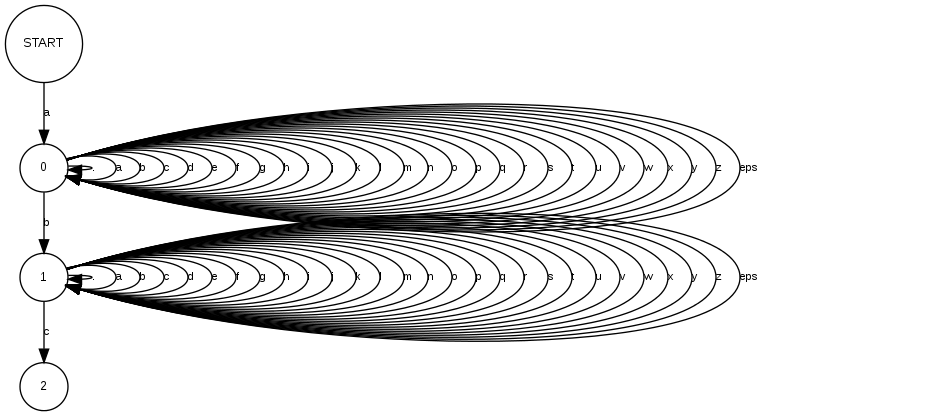
\includegraphics[height=3in]{a-star-b-star-c.png}
    \caption{NFA for regular expression \texttt{a.*b.*c} representing glob \texttt{a*b*c}
        over alphabet of lowercase letters and period (.)}
    \label{fig:nfaexample}
\end{figure}

\inputminted[fontsize=\footnotesize,linenos=true]{python}{code/ls.py}

\section{Parsing}

In programming problems, reading the input generally does not require parsing in the sense that
the syntactic structure of the input is given as a context-free grammar.  When it does, it is
usually part of the problem's challenge.  Though parsing, in general, is a wide topic area - 
the cases occurring in programming contests are usually simple grammars that describe a LL(1)
language, and the grammar is typically included in the problem's specification.

\subsection{Recursive Descent}

In a recursive descent parser, the structure of the code mirrors the structure of the grammar.
Non-terminals are represented by functions.
For instance, to read an equation which represents two expressions separated by a '=' terminal,
the grammar rule
\[
    Equation \rightarrow Expression = Expression
\]
would be implemented by a method such as this:

\inputminted[fontsize=\footnotesize,linenos=true]{python}{code/parseEquation.java}

\code{lookahead()} must peek at the next input token, but must not consume it.
A parser may call lookahead() multiple times before committing to a nonterminal and
consuming the token.
Generally, a recursive-descent parser's methods return a data structure that represents the
nonterminal implemented by that function.  Subtyping is commonly used to handle alternatives.

